\documentclass[12pt,a4paper]{article}
\usepackage[utf8x]{inputenc}
\usepackage{ucs}
\usepackage[spanish]{babel}
\usepackage{amsmath}
\usepackage{amsfonts}
\usepackage{amssymb}
\usepackage{makeidx}
\usepackage{graphicx}
\usepackage[hidelinks]{hyperref}
\usepackage[left=2cm,right=2cm,top=2cm,bottom=2cm]{geometry}
\author{Reyes Alvarez Ulises Isaac\\4.B   Ing. Mecatrónica\\Mtro. Carlos Enrique Morán Garabito\\Sistemas Electrónicos de Interfaz\\Sep - Dic 2019}
\title{Giro de un motor de corriente directa}
\begin{document}
\maketitle
\begin{figure}[hbtp]
\centering

\includegraphics[scale=2]{Circuitos/Universidad.png}
\end{figure}

\newpage
\section*{Motor de corriente directa (CD)}
Los motores de Corriente Directa o motor DC(correspondiente a las iniciales en inglés “direct current”) es también conocidos como motor de Corriente Continua o motor CC, son  muy utilizados en diseños de ingeniería debido a las características torque-velocidad que poseen con diferentes configuraciones eléctricas o mecánicas.\\
Una gran ventaja de los motores de CD se debe a que es posible controlarlos con suavidad y en la mayoría de los casos son reversibles, responden rápidamente gracias a que cuentan con una gran razón de torque a la inercia del rotor. Otra ventaja es la implementación del frenado dinámico, donde la energía generada por el motor se alimenta a un resistor disipador, y el frenado regenerativo donde la energía generada por el motor retroalimenta al suministro de potencia CD, esto es muy utilizado en aplicaciones donde se deseen frenados rápidos y de gran eficiencia.
\begin{figure}[hbtp]
\centering
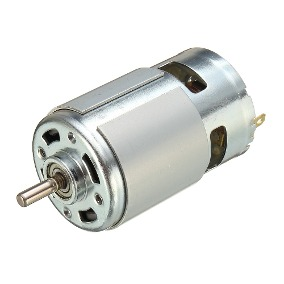
\includegraphics[scale=0.6]{Circuitos/Motor.jpg}
\caption{Motor de corriente directa}
\end{figure}

\section{Principio de funcionamiento}
El principio de funcionamiento de los motores eléctricos de corriente directa o continua se basa en la repulsión que ejercen los polos magnéticos de un imán permanente cuando, de acuerdo con la Ley de Lorentz, interactúan con los polos magnéticos de un electroimán que se encuentra montado en un eje. Este electroimán se denomina “rotor” y su eje le permite girar libremente entre los polos magnéticos norte y sur del imán permanente situado dentro de la carcasa o cuerpo del motor.\\
Cuando la corriente eléctrica circula por la bobina de este electroimán giratorio, el campo electromagnético que se genera interactúa con el campo magnético del imán permanente. Si los polos del imán permanente y del electroimán giratorio coinciden, se produce un rechazo y un torque magnético o par de fuerza que provoca que el rotor rompa la inercia y comience a girar sobre su eje en el mismo sentido de las manecillas del reloj en unos casos, o en sentido contrario, de acuerdo con la forma que se encuentre conectada al circuito la pila o la batería.

\newpage
\begin{figure}[hbtp]
\centering
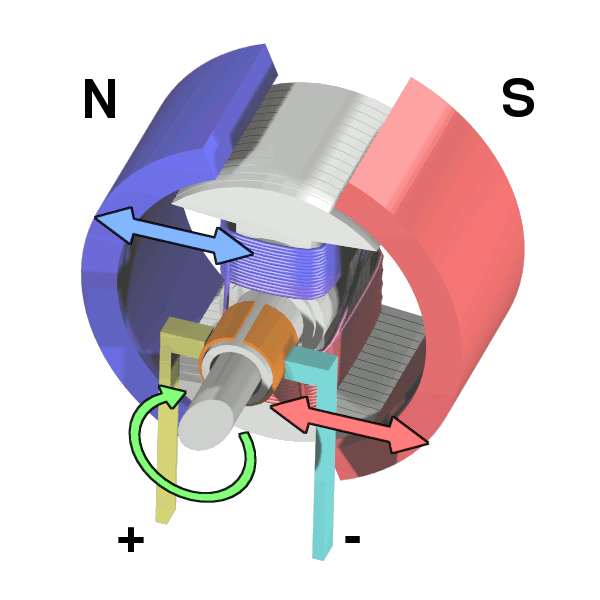
\includegraphics[scale=0.3]{Circuitos/Movimiento.png}
\caption{Movimiento de un motor de corriente directa}
\end{figure}
La siguiente figura muestra, de forma animada, el funcionamiento de un motor común bipolar de corriente directa. Como se puede observar, éste consta de un imán permanente en forma de semicírculo, dividido en dos partes fijas al cuerpo del motor. La parte de color rojo del imán corresponde al polo norte “N” y la azul al polo sur “S”. También encontramos un electro imán que a modo de rotor gira entre los polos magnéticos del imán permanente. En el eje del rotor se muestra un colector dividido en dos segmentos y dos escobillas haciendo contacto con los mismos. La batería se encuentra conectada de tal forma que la corriente eléctrica fluye en el sentido convencional con el polo positivo (+) conectado a la escobilla derecha y el polo negativo (–) a la escobilla izquierda. Cada escobilla hace pleno contacto con las secciones del colector, incluso mientras el rotor se encuentra girando.\\
Como la bobina del rotor se encuentra conectada a ambos segmentos del colector, éste se energiza con la corriente eléctrica directa que suministra la fuente de fuerza electromotriz (F.E.M.) (en este caso la batería), que le llega a través de las escobillas. De esa forma la corriente la recibe el colector a través de la escobilla izquierda identificada con el signo (+), recorre las espiras correspondientes a esa mitad de la bobina del electro imán (de color rojo) y continúa recorriendo las espiras de la mitad derecha (de color azul) para retornar, finalmente, a la batería por su polo negativo (–), completando así el circuito eléctrico del motor.\\
Cuando la corriente eléctrica comienza a fluir por la parte correspondiente a las espiras de color rojo, el electro imán adquiere polaridad norte “N” en ese extremo y polaridad sur “S” en el extremo opuesto representado por las espiras de color azul. 
De acuerdo con la Ley de Lorentz y aplicando “la regla de la mano izquierda” podremos comprobar que, en esas condiciones, el electro imán del rotor comienza a girar debido al torque magnético que se produce en sentido contrario a las manecillas del reloj. Dicho torque es resultado del rechazo que se manifiesta entre las polaridades magnéticas iguales del campo electromagnético del rotor y del campo magnético del imán permanente fijo en la carcasa del motor.\\
Cada vez que el electro imán del rotor da media vuelta y alcanza la posición vertical o neutra, los segmentos del colector (que giran también de forma conjunta con el rotor cambiando constantemente su posición), dejan de hacer contacto con las escobillas. En esa posición el suministro de corriente eléctrica a las espiras de la bobina cesa, por lo que el campo electromagnético desaparece por completo por unos instantes. La fuerza de inercia o impulso que mantiene el electro imán al llegar a la posición neutra permite que continúe girando y sobrepase ese punto de inmediato, por lo que los segmentos del colector pasan a ocupar la posición opuesta a la que tenían. En esta nueva posición la bobina se vuelve a energizar, pero al cambiar la polaridad de la corriente eléctrica que le suministra el colector, los polos magnéticos en cada extremo del electro imán del rotor también cambian.\\
El cambio constante de polaridad de la corriente en la bobina permite que los polos del electro imán sean siempre los mismos a cada lado del eje del rotor. Así pueden ser rechazados una y otra vez por los polos magnéticos del imán permanente, permitiendo que el rotor gire ininterrumpida mente durante todo el tiempo que la fuente de fuerza electromotriz (F.E.M.) se mantenga conectada al circuito eléctrico del motor.
Como se puede apreciar en la propia ilustración, de acuerdo con la forma en que se encuentra conectada la batería, el rotor gira en contra de las manecillas del reloj. Ahora bien, si queremos que gire en sentido contrario, sólo será necesario cambiar la conexión invirtiendo nosotros mismos su polaridad.\\
\begin{figure}[hbtp]
\centering
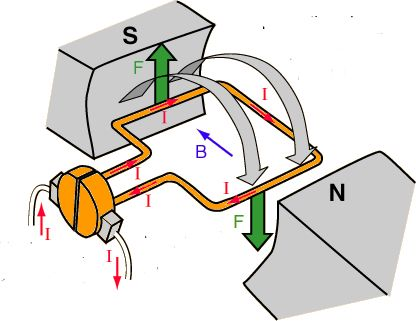
\includegraphics[scale=0.8]{Circuitos/Rotacion.jpg}
\caption{Rotacion Motor CC}
\end{figure}


\newpage
\section{Partes de un motor CC}
\begin{figure}[hbtp]
\centering
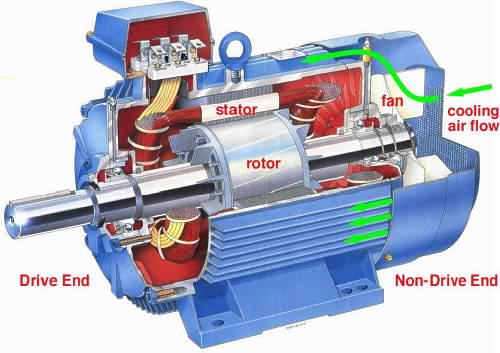
\includegraphics[scale=0.3]{Circuitos/Partes.jpg}
\caption{Partes de un motor de corriente directa}
\end{figure}

\subsubsection*{Carcasa metálica}
O cuerpo del motor. Aloja en su interior, de forma fija, dos imanes permanentes con forma de semicírculo, con sus correspondientes polos norte y sur.
\begin{figure}[hbtp]
\centering
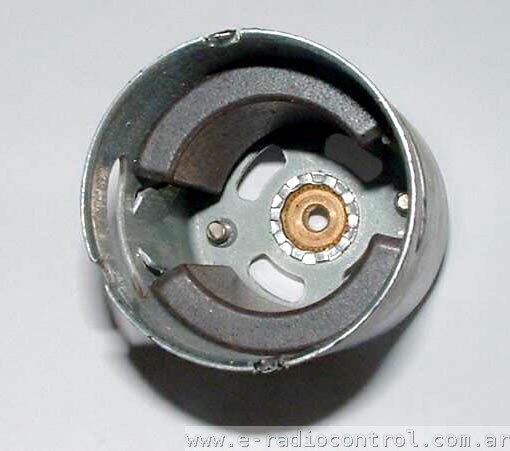
\includegraphics[scale=0.3]{Circuitos/carcasa.jpg}
\caption{Carcasa Motor CC}
\end{figure}

\subsubsection*{Rotor o parte giratoria del motor}
Se compone de una estructura metálica formada por un conjunto de chapas o láminas de acero al silicio, troqueladas con forma circular y montadas en un mismo eje con sus correspondientes bobinas de alambre de cobre, que lo convierten en un electro imán giratorio. Por norma general el rotor de la mayoría de los pequeños motores de C.D. se compone de tres enrollados o bobinas que crean tres polos magnéticos. Los extremos de cada una de esas bobinas se encuentran conectados a diferentes segmentos del colector.
\begin{figure}[hbtp]
\centering
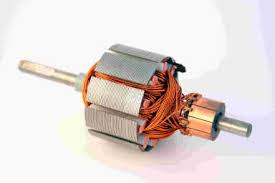
\includegraphics[scale=0.6]{Circuitos/rotor.jpg}
\caption{Rotor Motor CC}
\end{figure}

\subsection*{Colector o conmutador}
Situado en uno de los extremos del eje del rotor, se compone de un anillo deslizante seccionado en dos o más segmentos. Generalmente el colector de los pequeños motores comunes de C.D. se divide en tres segmentos.
\begin{figure}[hbtp]
\centering
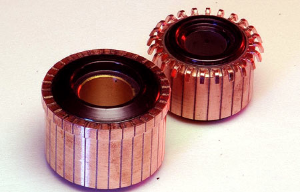
\includegraphics[scale=0.5]{Circuitos/conmutadores.png}
\caption{Conmutador Motor CC}
\end{figure}

\subsection*{Escobillas}
Representan dos contactos que pueden ser metálicos en unos casos, o compuesto por dos piezas de carbón en otros. Las escobillas constituyen contactos eléctricos que se deslizan por encima de los segmentos del colector mientras estos giran. Su misión es suministrar a la bobina o bobinas del rotor a través del colector, la corriente eléctrica directa necesaria para energizar el electro imán. En los pequeños motores las escobillas normalmente se componen de dos piezas o flejes metálicos que se encuentran fijos en la tapa que cierra la carcasa o cuerpo del motor.
\begin{figure}[hbtp]
\centering
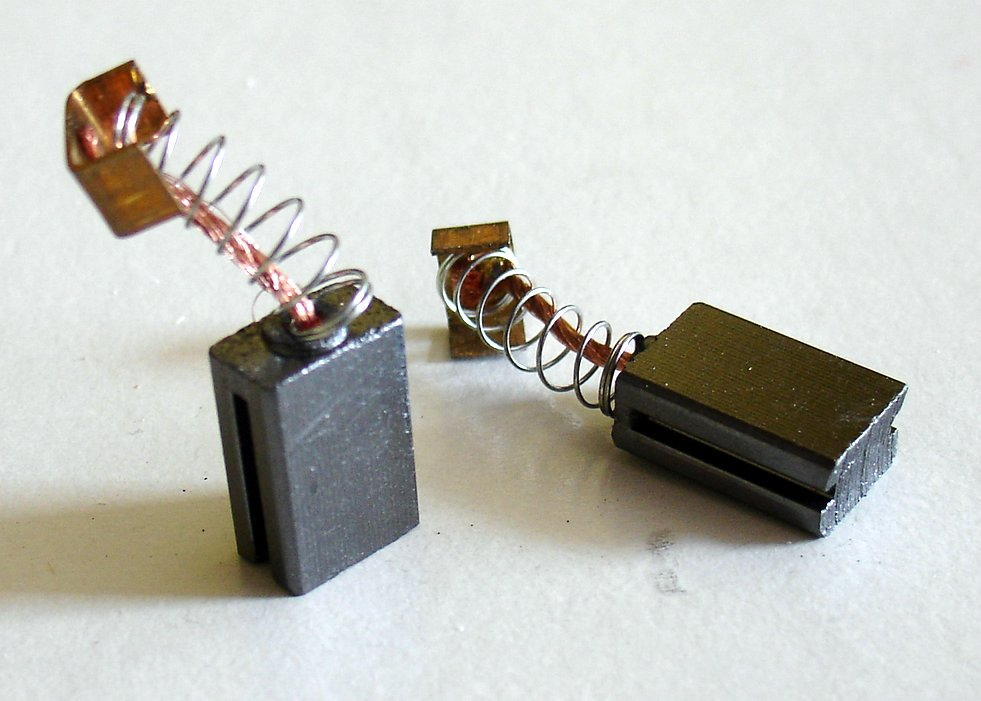
\includegraphics[scale=0.2]{Circuitos/escobillas.jpg}
\caption{Escobillas Motor CC}
\end{figure}

\subsection*{Tapa de la carcasa}
Es la tapa que se emplea para cerrar uno de los extremos del cuerpo o carcasa del motor. En su cara interna se encuentran situadas las escobillas de forma fija. El motor de esta foto utiliza en función de escobillas dos flejes metálicos.
\begin{figure}[hbtp]
\centering
\includegraphics[scale=0.6]{Circuitos/tapa.jpg}
\caption{Tapa de la carcasa Motor CC}
\end{figure}

\section{Referencias bibliográficas}
\url{http://www.asifunciona.com/electrotecnia/af_motor_cd/af_motor_cd_5.htm}\\
\url{https://www.mecatronicalatam.com/motores/motores-de-cd}\\

\end{document}